\section{Analyse des besoins}
Cette étape consiste à analyser et décortiquer les besoins pour en tirer une représentation en diagrammes formalisés.

\subsection{Identification des acteurs}
La première des missions est de bien identifier les acteurs qui vont interagir avec le système.\\
On entend par acteur, un humain, une machine, ou un système qui ne fait pas partie de la solution à réaliser mais qui participe au fonctionnement général de la solution par une interaction.\\
Dans notre cas nous avons des acteurs humains qui sont des collaborateurs.\\
Le but de la modélisation n'étant pas de reformuler forcément tous les détails de l'environnement d'un système, nous nous contenterons de spécifier en détail les points qui doivent l'être.\\
Ci-dessous les différents acteurs identifiés pour ce projet en détaillant leurs rôles

\begin{itemize}[label=\textbullet]
\item Administrateur : C'est l'acteur principal qui s'occupe du paramétrage et la gestion des utilisateurs, agences, profils et toutes autres fonctionnalités qui assurent le bon fonctionnement de l'application
\item Sous-administrateur : C'est un collaborateur défini par l'administrateur qui s'occupe du paramétrage ainsi que la gestion des ressources, droit d'accès et tous autres fonctionnalités spécifiques à son agence
\item Utilisateur : C'est un collaborateur ayant un droit défini par le sous-administrateur et qui interagit avec l'application selon son droit
\end{itemize}

\subsection{Diagramme de package}
Nous représentons à un niveau élevé d’abstraction les interactions des différents acteurs avec notre système.
\begin{figure}[h!]  
  \centering
    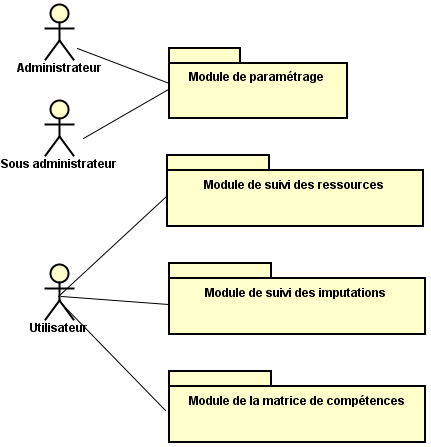
\includegraphics[width=0.7\textwidth]{chapitre2/Figures/package.png}
  \caption{Diagramme de package du système}
\end{figure}
\newpage
Comme présenté dans la figure ci-dessus, on a opté pour un découpage logique des modules afin d’avoir une vision plus claire sur le système. Dans ce cas, l'utilisateur aura accès à plusieurs modules présentés ci-dessus selon les droits attribués par l'administrateur, à savoir: le suivi des imputations, le suivi des ressources et la matrice de compétences. Ainsi l'administrateur et le sous-administrateur auront accès au paramétrage.
\subsection{Diagramme de cas d'utilisation}
Après avoir identifié les acteurs ainsi que les différents modules de notre application, il est nécessaire de déterminer pour
chaque module les cas d’utilisation qui lui sont dédiés.\\
Les cas d’utilisation permettent de représenter le fonctionnement du système vis-à-vis de l’utilisateur : c’est donc une vue du système dans son environnement extérieur. Dans ce qui suit on va décortiquer chaque module et ces cas d'utilisation.\\

\subsubsection{Module de paramétrage}
\begin{figure}[h!]  
  \centering
    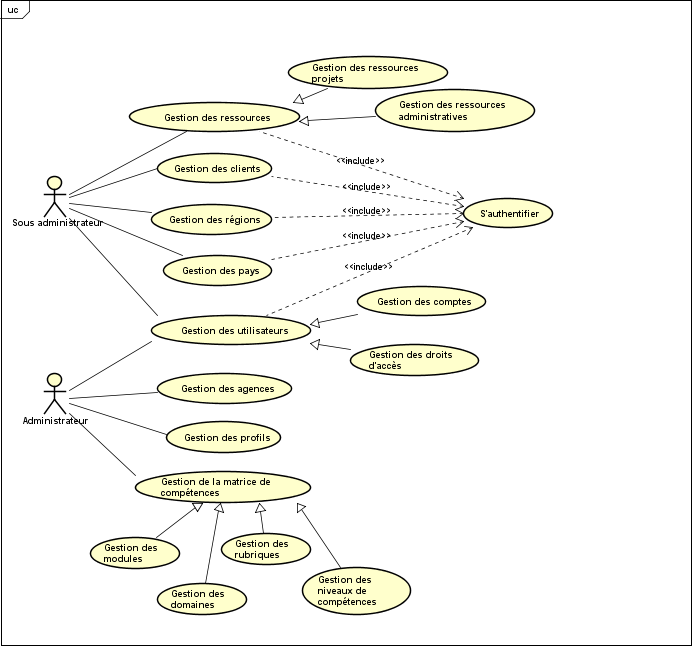
\includegraphics[width=0.95\textwidth]{chapitre2/Figures/parametrageUC.png}
  \caption{Diagramme de cas d’utilisation du module paramétrage}
\end{figure}
\newpage
\subsubsection*{Description des cas d’utilisations }
\begin{itemize}[label=\textbullet]
%Gestion des actions demandées
\item \textbf{Gestion des actions demandées :}
\begin{table}[!h]
\begin{tabular}{|p{15cm}|}%p{2.5cm}|p{9cm}
\rowcolor{shadecolor}\multicolumn{1}{|c|}{Sommaire d’indentification} \\
\hline
\textbf{objectif : } cette fonctionnalité permet de gérer les actions demandées\\
\textbf{acteurs : } administrateur\\
\textbf{précondition : } l'acteur est connecté au système\\
\hline
\rowcolor{shadecolor}\multicolumn{1}{|c|}{Description des scénarios} \\
\hline
	\textbf{Scénario nominal :}
	\begin{itemize}[label=\textbullet]
	\item scénario "ajouter action" :
		\begin{itemize}
		\item l'acteur ouvre le formulaire d'ajout
		\item l'acteur saisie les champs de l'action'
		\item l'acteur confirme l'ajout
		\item le système enregistre les données
		\end{itemize}
	\item scénario "modifier action" :
		\begin{itemize}
		\item l'acteur affiche la liste des actions
		\item l'acteur sélectionne l'action à modifier
		\item le système affiche les informations de l'action sélectionnée
		\item l'acteur modifie les champs ciblés
		\item l'acteur valide ses modifications
		\item le système confirme la modification
		\end{itemize}
	\item scénario "supprimer action" :
		\begin{itemize}
		\item l'acteur affiche la liste des actions
		\item l'acteur sélectionne l'action à supprimer
		\item le système affiche un message de confirmation
		\item l'acteur confirme la suppression
		\item le système supprime l'action'
		\end{itemize}
	\end{itemize}
	\textbf{Scénario Alternatives  :}\\
	Le système vérifie si l'action existe déjà dans la BD avant l’ajout.\\
\hline
\end{tabular}
\centering \caption{Description du cas d’utilisation "Gestion des actions demandées"} \label{TablePR}
\end{table}
%Gestion des états d'action
\newpage
\item \textbf{Gestion des états d'action :}\\
\begin{table}[!h]
\begin{tabular}{|p{15cm}|}%p{2.5cm}|p{9cm}
\rowcolor{shadecolor}\multicolumn{1}{|c|}{Sommaire d’indentification} \\
\hline
\textbf{objectif : } cette fonctionnalité permet de gérer les états d'action\\
\textbf{acteurs : } administrateur\\
\textbf{précondition : } l'acteur est connecté au système\\
\hline
\rowcolor{shadecolor}\multicolumn{1}{|c|}{Description des scénarios} \\
\hline
	\textbf{Scénario nominal :}
	\begin{itemize}[label=\textbullet]
	\item scénario "ajouter état" :
		\begin{itemize}
		\item l'acteur ouvre le formulaire d'ajout
		\item l'acteur saisie les champs d'état
		\item l'acteur confirme l'ajout
		\item le système enregistre les données
		\end{itemize}
	\item scénario "modifier état" :
		\begin{itemize}
		\item l'acteur affiche la liste des états
		\item l'acteur sélectionne l'état à modifier
		\item le système affiche les informations d'état sélectionnée
		\item l'acteur modifie les champs ciblés
		\item l'acteur valide ses modifications
		\item le système confirme la modification
		\end{itemize}
	\item scénario "supprimer état" :
		\begin{itemize}
		\item l'acteur affiche la liste des états
		\item l'acteur sélectionne l'état à supprimer
		\item le système affiche un message de confirmation
		\item l'acteur confirme la suppression
		\item le système supprime l'état
		\end{itemize}
	\end{itemize}
	\textbf{Scénario Alternatives  :}\\
	Le système vérifie si l'état existe déjà dans la BD avant l’ajout.\\
\hline
\end{tabular}
\centering \caption{Description du cas d’utilisation "Gestion des états d'action"} \label{TablePR}
\end{table}

%Gestion des états des composants
\newpage
\item \textbf{Gestion des états des composants :}\\
\begin{table}[!h]
\begin{tabular}{|p{15cm}|}%p{2.5cm}|p{9cm}
\rowcolor{shadecolor}\multicolumn{1}{|c|}{Sommaire d’indentification} \\
\hline
\textbf{objectif : } cette fonctionnalité permet de gérer les états des composants\\
\textbf{acteurs : } administrateur\\
\textbf{précondition : } l'acteur est connecté au système\\
\hline
\rowcolor{shadecolor}\multicolumn{1}{|c|}{Description des scénarios} \\
\hline
	\textbf{Scénario nominal :}
	\begin{itemize}[label=\textbullet]
	\item scénario "ajouter état" :
		\begin{itemize}
		\item l'acteur ouvre le formulaire d'ajout
		\item l'acteur saisie les champs d'état
		\item l'acteur confirme l'ajout
		\item le système enregistre les données
		\end{itemize}
	\item scénario "modifier état" :
		\begin{itemize}
		\item l'acteur affiche la liste des états
		\item l'acteur sélectionne l'état à modifier
		\item le système affiche les informations d'état sélectionnée
		\item l'acteur modifie les champs ciblés
		\item l'acteur valide ses modifications
		\item le système confirme la modification
		\end{itemize}
	\item scénario "supprimer état" :
		\begin{itemize}
		\item l'acteur affiche la liste des états
		\item l'acteur sélectionne l'état à supprimer
		\item le système affiche un message de confirmation
		\item l'acteur confirme la suppression
		\item le système supprime l'état
		\end{itemize}
	\end{itemize}
	\textbf{Scénario Alternatives  :}\\
	Le système vérifie si l'état existe déjà dans la BD avant l’ajout.\\
\hline
\end{tabular}
\centering \caption{Description du cas d’utilisation "Gestion des états des composants"} \label{TablePR}
\end{table}


\end{itemize}
\newpage
\subsubsection{Module opération}
\begin{figure}[h!]  
  \centering
    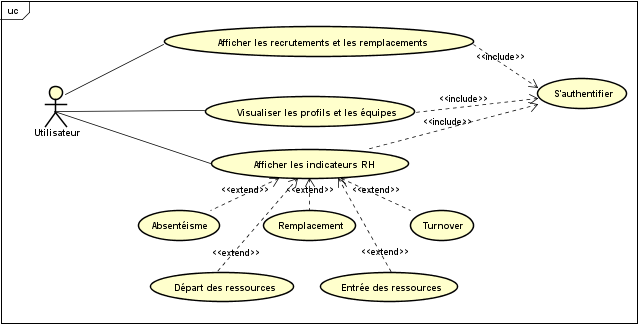
\includegraphics[width=0.95\textwidth]{chapitre2/Figures/ressourcesUC.png}
  \caption{Diagramme de cas d’utilisation du module de suivi des ressources}
\end{figure}
\subsubsection*{Description des cas d’utilisations }
\begin{itemize}[label=\textbullet]

%Afficher les groupes des TPE
\item \textbf{Afficher les groupes des TPE :}
\begin{table}[!h]
\begin{tabular}{|p{15cm}|}%p{2.5cm}|p{9cm}
\rowcolor{shadecolor}\multicolumn{1}{|c|}{Sommaire d’indentification} \\
\hline
\textbf{objectif : } cette fonctionnalité permet d'fficher les groupes des TPE\\
\textbf{acteurs : } utilisateur\\
\textbf{précondition : } 
	\begin{itemize}[label=\textbullet]
	\item l'acteur est connecté au système
	\item l'acteur a le droit d'accès
	\end{itemize}
	\\
\hline
\rowcolor{shadecolor}\multicolumn{1}{|c|}{Description des scénarios} \\
\hline
	\textbf{Scénario nominal :}
	\begin{itemize}[label=\textbullet]
	\item scénario "Afficher les groupe des TPE" :
		\begin{itemize}
		\item l'acteur demande de visualiser l'ensemble des groupes des TPE
		\item le système affiche un tableau contenant l'ensemble des groupes des TPE.
		\end{itemize}
	\end{itemize}
	\\
\hline
\end{tabular}
\centering \caption{Description du cas d’utilisation "Afficher les groupes des TPE"} \label{TablePR}
\end{table}

\newpage
%Visulaliser tous les TPE par groupe
\item \textbf{Visulaliser la liste des TPE par goupe :}
\begin{table}[!h]
\begin{tabular}{|p{15cm}|}%p{2.5cm}|p{9cm}
\rowcolor{shadecolor}\multicolumn{1}{|c|}{Sommaire d’indentification} \\
\hline
\textbf{objectif : } cette fonctionnalité permet de visualiser la liste des TPE affiché par groupe\\
\textbf{acteurs : } utilisateur\\
\textbf{précondition : } 
	\begin{itemize}[label=\textbullet]
	\item l'acteur est connecté au système
	\item l'acteur a le droit d'accès
	\end{itemize}
	\\
\hline
\rowcolor{shadecolor}\multicolumn{1}{|c|}{Description des scénarios} \\
\hline
	\textbf{Scénario nominal :}
	\begin{itemize}[label=\textbullet]
	\item scénario "Visulaliser la liste des TPE" :
		\begin{itemize}
		\item le système affiche l'ensemble des TPE regroupés par groupes
		\end{itemize}
	\end{itemize}
	\\
\hline
\end{tabular}
\centering \caption{Description du cas d’utilisation "visualiser la liste des TPE affiché par groupe"} \label{TablePR}
\end{table}

%Afficher les TPE d'un seule groupe
\item \textbf{Afficher les TPE d'un groupe :}
\begin{table}[!h]
\begin{tabular}{|p{15cm}|}%p{2.5cm}|p{9cm}
\rowcolor{shadecolor}\multicolumn{1}{|c|}{Sommaire d’indentification} \\
\hline
\textbf{objectif : } cette fonctionnalité permet d'afficher la liste des TPE d'un groupe\\
\textbf{acteurs : } utilisateur\\
\textbf{précondition : } 
	\begin{itemize}[label=\textbullet]
	\item l'acteur est connecté au système
	\item l'acteur a le droit d'accès
	\end{itemize}
	\\
\hline
\rowcolor{shadecolor}\multicolumn{1}{|c|}{Description des scénarios} \\
\hline
	\textbf{Scénario nominal :}
	\begin{itemize}[label=\textbullet]
	\item scénario "Afficher les TPE d'un groupe" :
		\begin{itemize}
		\item le système affiche l'ensemble des TPE du groupe
	
		\end{itemize}
	\end{itemize}
	\\
\hline
\end{tabular}
\centering \caption{Description du cas d’utilisation "Afficher les TPE d'un groupe"} \label{TablePR}
\end{table}

%Chercher un groupe des TPE 
\newpage
\item \textbf{Chercher un groupe des TPE :}
\begin{table}[!h]
\begin{tabular}{|p{15cm}|}%p{2.5cm}|p{9cm}
\rowcolor{shadecolor}\multicolumn{1}{|c|}{Sommaire d’indentification} \\
\hline
\textbf{objectif : } cette fonctionnalité permet de chercher un groupe des TPE \\
\textbf{acteurs : } utilisateur\\
\textbf{précondition : } 
	\begin{itemize}[label=\textbullet]
	\item l'acteur est connecté au système
	\item l'acteur a le droit d'accès
	\end{itemize}
	\\
\hline
\rowcolor{shadecolor}\multicolumn{1}{|c|}{Description des scénarios} \\
\hline
	\textbf{Scénario nominal :}
	\begin{itemize}[label=\textbullet]
	\item scénario "Chercher un groupe des TPE" :
		\begin{itemize}
		\item l'acteur saisie les critères de recherche dans dans les champs de saisie
		\item le système filtre les données selon : code du groupe, nom du banque
		\item le système affiche le groupe cherché
	
		\end{itemize}
	\end{itemize}
	\\
\hline
\end{tabular}
\centering \caption{Description du cas d’utilisation "Chercher un groupe des TPE"} \label{TablePR}
\end{table}

%Chercher un TPE 
\item \textbf{Chercher un TPE :}
\begin{table}[!h]
\begin{tabular}{|p{15cm}|}%p{2.5cm}|p{9cm}
\rowcolor{shadecolor}\multicolumn{1}{|c|}{Sommaire d’indentification} \\
\hline
\textbf{objectif : } cette fonctionnalité permet de chercher un TPE \\
\textbf{acteurs : } utilisateur\\
\textbf{précondition : } 
	\begin{itemize}[label=\textbullet]
	\item l'acteur est connecté au système
	\item l'acteur a le droit d'accès
	\end{itemize}
	\\
\hline
\rowcolor{shadecolor}\multicolumn{1}{|c|}{Description des scénarios} \\
\hline
	\textbf{Scénario nominal :}
	\begin{itemize}[label=\textbullet]
	\item scénario "Chercher un TPE" :
		\begin{itemize}
		\item l'acteur saisie les critères de recherche dans dans les champs de saisie
		\item le système filtre les données selon : code du TPE, code du groupe, nom du banque
		\item le système affiche le TPE cherché
	
		\end{itemize}
	\end{itemize}
	\\
\hline
\end{tabular}
\centering \caption{Description du cas d’utilisation "Chercher un TPE"} \label{TablePR}
\end{table}

%Configurer les informations demandées 
\item \textbf{Configurer les informations demandées du TPE :}
\begin{table}[!h]
\begin{tabular}{|p{15cm}|}%p{2.5cm}|p{9cm}
\rowcolor{shadecolor}\multicolumn{1}{|c|}{Sommaire d’indentification} \\
\hline
\textbf{objectif : } cette fonctionnalité permet l'acteur de demander l'ensemble des informations du TPE \\
\textbf{acteurs : } utilisateur\\
\textbf{précondition : } 
	\begin{itemize}[label=\textbullet]
	\item l'acteur est connecté au système
	\item l'acteur a le droit d'accès
	\end{itemize}
	\\
\hline
\rowcolor{shadecolor}\multicolumn{1}{|c|}{Description des scénarios} \\
\hline
	\textbf{Scénario nominal :}
	\begin{itemize}[label=\textbullet]
	\item scénario "Configurer les informations demandées du TPE" :
		\begin{itemize}
		\item l'acteur précise les informations demandées du TPE
		\item le système filtre enregistre l'ensemble des informations demandées.
	
		\end{itemize}
	\end{itemize}
	\\
\hline
\end{tabular}
\centering \caption{Description du cas d’utilisation "Configurer les informations demandées du TPE"} \label{TablePR}
\end{table}




\end{itemize}
\newpage
\subsubsection{Module d'exploitation des données}
\begin{figure}[h!]  
  \centering
    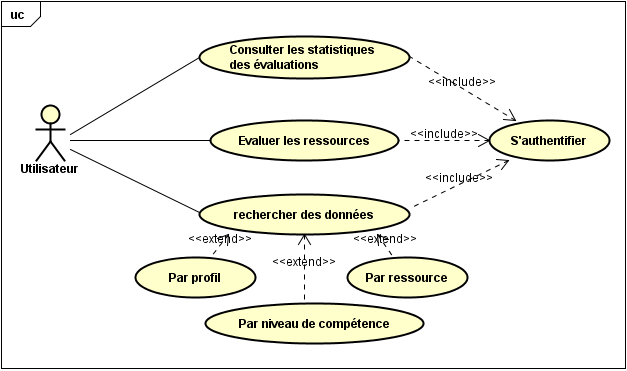
\includegraphics[width=0.95\textwidth]{chapitre2/Figures/competencesUC.png}
  \caption{Diagramme de cas d’utilisation du module de la matrice de comptétences}
\end{figure}
\subsubsection*{Description des cas d’utilisations }
\begin{itemize}[label=\textbullet]
\newpage
%Consulter l'état matériel
\item \textbf{Consulter l'état d'un TPE :}
\begin{table}[!h]
\begin{tabular}{|p{15cm}|}%p{2.5cm}|p{9cm}
\rowcolor{shadecolor}\multicolumn{1}{|c|}{Sommaire d’indentification} \\
\hline
\textbf{objectif : } cette fonctionnalité permet de visualiser les informations concernant l'état en temps réel du TPE \\
\textbf{acteurs : } utilisateur\\
\textbf{précondition : } 
	\begin{itemize}[label=\textbullet]
	\item l'acteur est connecté au système
	\item l'acteur a le droit d'accès
	\end{itemize}
	\\
\hline
\rowcolor{shadecolor}\multicolumn{1}{|c|}{Description des scénarios} \\
\hline
	\textbf{Scénario nominal :}
	\begin{itemize}[label=\textbullet]
	\item scénario "Consulter l'état d'un TPE" :
		\begin{itemize}
		\item l'acteur demande de visualiser les informations de l'état du TPE
		\item le système regroupe l'ensemble des informations demandées 
		
		\item le système affiche les informations du TPE et des tableaux qui synthétise l'état matériel et logiciel du TPE
		\end{itemize}
	\end{itemize}
	\\
\hline
\end{tabular}
\centering \caption{Description du cas d’utilisation "Consulter l'état d'un TPE"} \label{TablePR}
\end{table}



\newpage
%Consulter les statistiques d'un groupe de TPE
\item \textbf{Consulter les statistiques d'un groupe de TPE :}
\begin{table}[!h]
\begin{tabular}{|p{15cm}|}%p{2.5cm}|p{9cm}
\rowcolor{shadecolor}\multicolumn{1}{|c|}{Sommaire d’indentification} \\
\hline
\textbf{objectif : } cette fonctionnalité permet de visualiser  les statistiques d'un groupe de TPE \\
\textbf{acteurs : } utilisateur\\
\textbf{précondition : } 
	\begin{itemize}[label=\textbullet]
	\item l'acteur est connecté au système
	\item l'acteur a le droit d'accès
	\end{itemize}
	\\
\hline
\rowcolor{shadecolor}\multicolumn{1}{|c|}{Description des scénarios} \\
\hline
	\textbf{Scénario nominal :}
	\begin{itemize}[label=\textbullet]
	\item scénario "Consulter les statistiques d'un groupe de TPE" :
		\begin{itemize}
		\item l'acteur sélectionne un groupe de TPE
		\item le système affiche la liste des TPE et des champs de dates et de choix d'unité de temps
		\item l'acteur sélectionne : l'ensemble des TPE,date début, date fin, l'unité de temps(jours,mois)
		\item l'acteur lance la recherche
		\item le système affiche des champs, tableaux et des graphes qui synthétisent l'ensemble des statistiques.
		\end{itemize}
	\end{itemize}
	\\
\hline
\end{tabular}
\centering \caption{Consulter les statistiques d'un groupe de TPE"} \label{TablePR}
\end{table}



\end{itemize}

